\documentclass[11pt]{article}
\usepackage[utf8]{inputenc}
\usepackage[T1]{fontenc}
\usepackage{amsmath,amssymb}
\usepackage{graphicx}
\usepackage{xcolor}
\usepackage{booktabs}
\usepackage[margin=2.1cm]{geometry}
\usepackage{array}
\usepackage{fancyhdr}

\definecolor{azul}{RGB}{0,70,140}

\newcommand{\seccion}[1]{%
  \vspace{4pt}\noindent{\color{azul}\large\bfseries #1}\par\vspace{2pt}\hrule\vspace{6pt}}

\pagestyle{fancy}\fancyhf{}
\rhead{\small Modelado y Simulación}
\lhead{\small Resolución de examen — Parte 3}
\cfoot{\thepage}

\setlength{\parindent}{0pt}
\setlength{\parskip}{4pt}

\begin{document}

\begin{center}
  {\color{azul}\LARGE\bfseries Resolución completa del examen (Parte 3)}\\[2pt]
  {\large Integración numérica · Competencia · Van der Pol · Modelo SIR}\\[2pt]
  \rule{\textwidth}{0.8pt}
\end{center}

%==================================================================
\seccion{Ejercicio 1 — Integración numérica de $\displaystyle\int_0^1 \frac{\ln(x+1)}{x}\,dx$}

\textbf{Nota sobre la singularidad.} En $x=0$ el integrando es indeterminado $\tfrac00$, pero tiene
límite finito:
\[
\lim_{x\to0}\frac{\ln(1+x)}{x}=1\quad(\text{regla de L'Hôpital o serie }\ln(1+x)=x-\tfrac{x^2}{2}+\dots).
\]
Por eso tomamos $f(0)=1$. Con $n=4$ subintervalos: $h=\dfrac{1-0}{4}=0.25$.

\textbf{Tabla de valores} $f(x_i)=\dfrac{\ln(1+x_i)}{x_i}$:
\begin{center}
\renewcommand{\arraystretch}{1.25}
\begin{tabular}{c c c c}
\toprule
$i$ & $x_i$ & $\ln(1+x_i)$ & $f(x_i)$\\
\midrule
0 & 0.00 & 0.000000 & $1.000000$ (límite)\\
1 & 0.25 & 0.223144 & $0.892574$\\
2 & 0.50 & 0.405465 & $0.810930$\\
3 & 0.75 & 0.559616 & $0.746154$\\
4 & 1.00 & 0.693147 & $0.693147$\\
\bottomrule
\end{tabular}
\end{center}

\textbf{a) Regla del trapecio compuesta.}
\[
T=\frac{h}{2}\Big[f_0+2\big(f_1+f_2+f_3\big)+f_4\Big].
\]
\[
f_1+f_2+f_3=0.892574+0.810930+0.746154=2.449659.
\]
\[
T=\frac{0.25}{2}\big[\,1+2(2.449659)+0.693147\,\big]
=0.125\cdot 6.592465=\boxed{0.824058}.
\]

\textbf{b) Regla de Simpson $1/3$ compuesta} ($n=4$ par):
\[
S=\frac{h}{3}\Big[f_0+4\big(f_1+f_3\big)+2f_2+f_4\Big].
\]
\[
4(f_1+f_3)=4(0.892574+0.746154)=4(1.638729)=6.554915,\qquad 2f_2=1.621860.
\]
\[
S=\frac{0.25}{3}\big[\,1+6.554915+1.621860+0.693147\,\big]
=0.083333\cdot 9.869922=\boxed{0.822493}.
\]

\textbf{Tabla resumen} (valor exacto $=\dfrac{\pi^2}{12}=0.822467$):
\begin{center}
\renewcommand{\arraystretch}{1.25}
\begin{tabular}{l c c}
\toprule
Método & Aproximación & Error absoluto\\
\midrule
Trapecio ($n=4$)     & $0.824058$ & $1.59\times10^{-3}$\\
Simpson $1/3$ ($n=4$)& $0.822493$ & $2.65\times10^{-5}$\\
Exacto ($\pi^2/12$)  & $0.822467$ & --\\
\bottomrule
\end{tabular}
\end{center}
Simpson es $\sim\!60$ veces más preciso que el trapecio (usa parábolas en lugar de rectas).

\newpage
%==================================================================
\seccion{Ejercicio 2 — Sistema no lineal con parámetro $\mu$}

Reescribimos el sistema factorizando:
\[
\begin{cases}
\dot x=x(2-x)-xy=\ x\,(2-x-y)\\[2pt]
\dot y=y(1-y)-xy+\mu y=\ y\,(1+\mu-x-y)
\end{cases}
\]
Es un modelo de \textbf{competencia} (tipo Lotka–Volterra): $x$ tiene capacidad $2$ y $y$ capacidad $1+\mu$.

\textbf{a) Nulclinas y regiones.}
\[
\dot x=0:\ \ \boxed{x=0}\ \ \text{ó}\ \ \boxed{x+y=2};\qquad
\dot y=0:\ \ \boxed{y=0}\ \ \text{ó}\ \ \boxed{x+y=1+\mu}.
\]
Las dos rectas $x+y=2$ y $x+y=1+\mu$ tienen \emph{pendiente $-1$} (son paralelas): solo se cortan si
$2=1+\mu$, es decir $\mu=1$. Por eso \textbf{no hay punto de coexistencia interior} salvo en el caso
crítico $\mu=1$ (donde toda la recta $x+y=2$ queda de equilibrios).

\textbf{Puntos de equilibrio} (para $\mu\neq1$):
\[
\boxed{(0,0)},\qquad \boxed{(2,0)},\qquad \boxed{(0,\,1+\mu)}.
\]

\textbf{b) Linealización.} Jacobiano ($\dot x=2x-x^2-xy,\ \dot y=(1+\mu)y-y^2-xy$):
\[
J(x,y)=\begin{pmatrix} 2-2x-y & -x\\ -y & 1+\mu-2y-x\end{pmatrix}.
\]
\[
J(0,0)=\begin{pmatrix}2&0\\0&1+\mu\end{pmatrix}\Rightarrow \lambda=2,\ 1+\mu>0
\ \Rightarrow\ \boxed{(0,0)\ \text{NODO INESTABLE}}.
\]
\[
J(2,0)=\begin{pmatrix}-2&-2\\0&\mu-1\end{pmatrix}\Rightarrow \lambda=-2,\ \mu-1.
\]
\[
J(0,1+\mu)=\begin{pmatrix}1-\mu&0\\-(1+\mu)&-(1+\mu)\end{pmatrix}\Rightarrow \lambda=1-\mu,\ -(1+\mu).
\]

\textbf{Topología según $\mu$ y bifurcación.} El signo de $\mu-1$ decide todo:
\begin{center}\small
\renewcommand{\arraystretch}{1.3}
\begin{tabular}{c l l l}
\toprule
Caso & $(2,0)$ & $(0,1+\mu)$ & Resultado\\
\midrule
$\mu<1$ & $\lambda=-2,\mu\!-\!1<0$: \textbf{nodo estable} & $\lambda=1\!-\!\mu>0$: \textbf{silla} & gana $x$ (conejos)\\
$\mu=1$ & $\lambda=-2,0$: degenerado & $\lambda=0,-2$: degenerado & recta de equilibrios $x{+}y{=}2$\\
$\mu>1$ & $\lambda=-2,\mu\!-\!1>0$: \textbf{silla} & $\lambda=1\!-\!\mu<0$: \textbf{nodo estable} & gana $y$ (ovejas)\\
\bottomrule
\end{tabular}
\end{center}
En $\mu=1$ un autovalor de cada equilibrio de borde cruza por $0$: es una \textbf{bifurcación
transcrítica} (intercambio de estabilidad). Para $\mu<1$ prevalece $x$; para $\mu>1$ prevalece $y$;
en $\mu=1$ hay empate (capacidades iguales, $2=1+\mu$).

\begin{figure}[htbp]\centering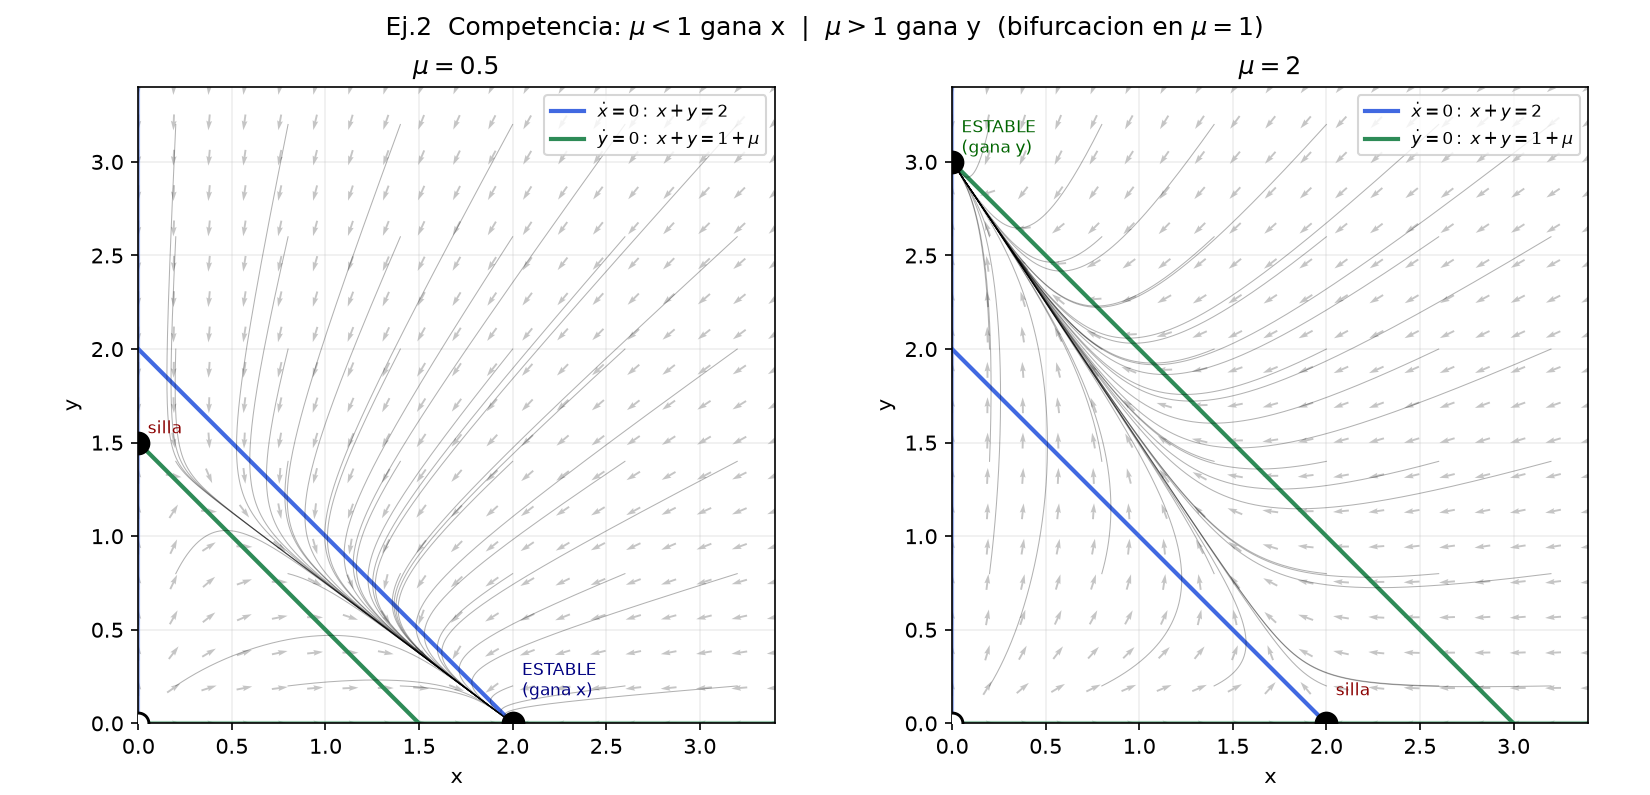
\includegraphics[width=0.99\textwidth]{ej2b_nulclinas.png}\end{figure}

\newpage
%==================================================================
\seccion{Ejercicio 3 — Oscilador de Van der Pol}

\[
\ddot x-\mu(1-x^2)\dot x+x=0,\qquad \mu>0.
\]

\textbf{a) Forma de estado 2D.} Con $x_1=x,\ x_2=\dot x$:
\[
\boxed{\ \begin{cases}\dot x_1=x_2\\[2pt] \dot x_2=\mu(1-x_1^2)\,x_2-x_1\end{cases}\ }
\]
\textbf{Equilibrio.} $\dot x_1=0\Rightarrow x_2=0$; $\dot x_2=0\Rightarrow x_1=0$. Único: $(0,0)$.

\textbf{Linealización.} Jacobiano:
\[
J(x_1,x_2)=\begin{pmatrix}0 & 1\\ -2\mu x_1 x_2-1 & \mu(1-x_1^2)\end{pmatrix}
\ \Rightarrow\
J(0,0)=\begin{pmatrix}0&1\\-1&\mu\end{pmatrix}.
\]
\[
\operatorname{tr}=\mu>0,\qquad \det=1>0,\qquad
\lambda=\frac{\mu\pm\sqrt{\mu^2-4}}{2}.
\]
\begin{itemize}
  \item $0<\mu<2$: raíces complejas con parte real $\mu/2>0$ $\Rightarrow$ \textbf{foco (espiral) inestable}.
  \item $\mu=2$: raíz doble $\lambda=1>0$ $\Rightarrow$ nodo inestable degenerado.
  \item $\mu>2$: dos raíces reales positivas $\Rightarrow$ \textbf{nodo inestable}.
\end{itemize}
En todos los casos ($\mu>0$) el origen es \textbf{inestable}.

\textbf{Comportamiento cualitativo — ciclo límite.} El término $-\mu(1-x^2)\dot x$ actúa como un
\emph{amortiguamiento variable}:
\begin{itemize}
  \item Para $|x|<1$: el coeficiente $-\mu(1-x^2)<0$ es \emph{amortiguamiento negativo} $\Rightarrow$
        inyecta energía y las trayectorias \textbf{salen} en espiral desde el origen.
  \item Para $|x|>1$: el coeficiente es positivo $\Rightarrow$ disipa energía y las trayectorias
        \textbf{entran}.
\end{itemize}
El equilibrio entre inyección y disipación produce un \textbf{ciclo límite estable único}: toda
órbita (salvo el punto fijo) tiende a él. Es un \emph{oscilador autosostenido}. Para $\mu$ grande el
ciclo toma forma de \emph{oscilaciones de relajación} (tramos lentos y saltos rápidos).

\textbf{b) Retrato de estado.}
\begin{figure}[htbp]\centering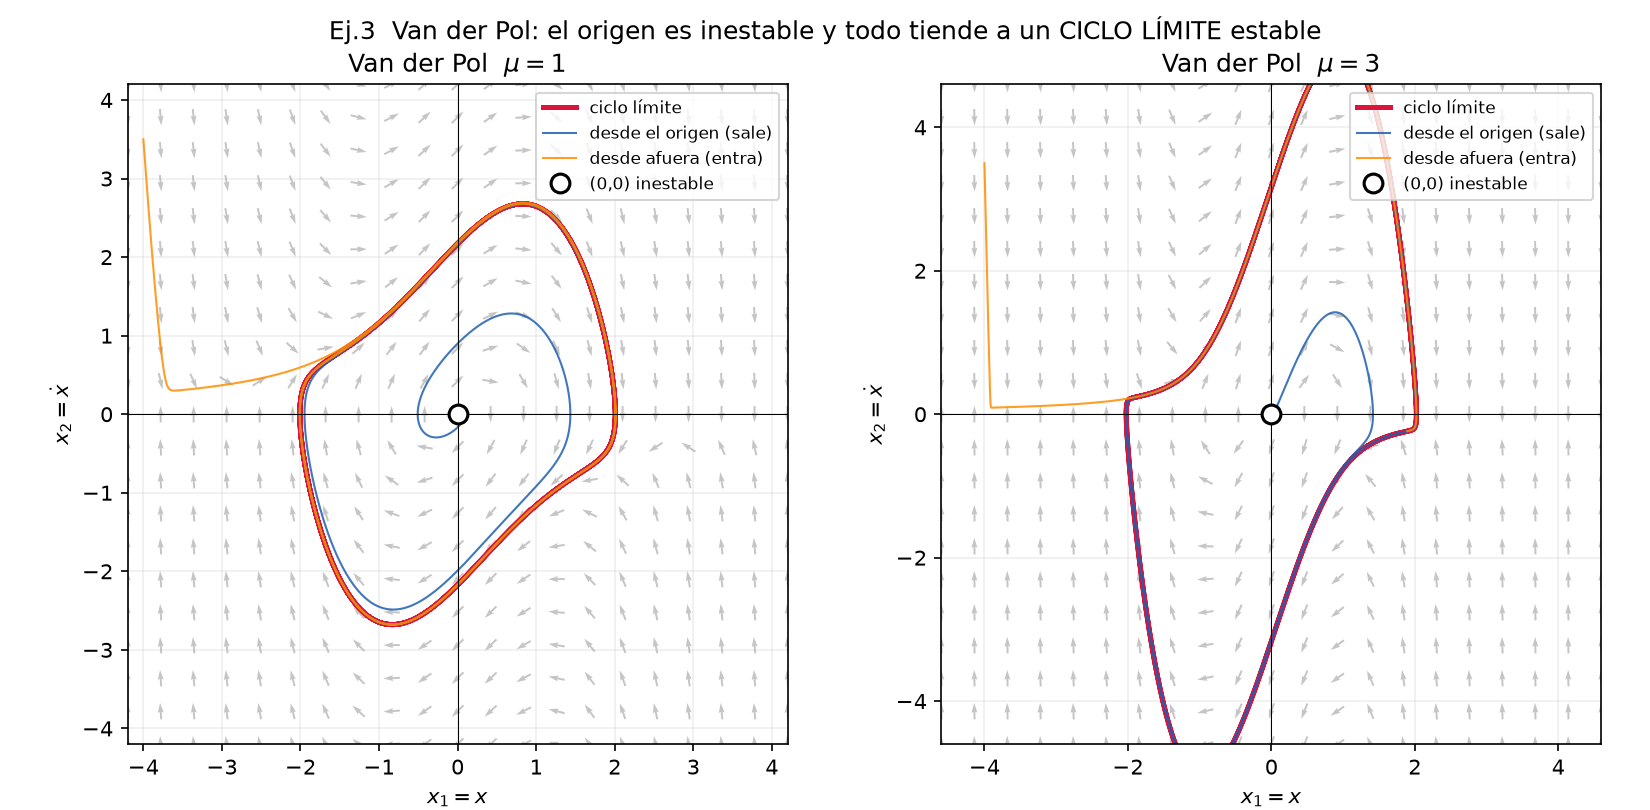
\includegraphics[width=0.99\textwidth]{ej3b_vanderpol.png}\end{figure}

\newpage
%==================================================================
\seccion{Ejercicio 4 — Modelo epidémico SIR}

\[
\begin{cases}\dot S=-\alpha S I\\[2pt]\dot I=\alpha S I-\beta I\\[2pt]\dot R=\beta I\end{cases}
\qquad S_0=25,\ I_0=3,\ \alpha=0.2,\ \beta=5.
\]
La población total es constante: $\dot S+\dot I+\dot R=0\Rightarrow N=S+I+R=28$.

\textbf{a) ``Resolver'' — trayectoria en el plano $S\!-\!I$.} No hay solución cerrada en $t$, pero
dividiendo las dos primeras ecuaciones se elimina el tiempo:
\[
\frac{dI}{dS}=\frac{\alpha S I-\beta I}{-\alpha S I}=\frac{\alpha S-\beta}{-\alpha S}=-1+\frac{\beta}{\alpha S}.
\]
Integrando:
\[
I(S)=-S+\frac{\beta}{\alpha}\ln S+C,\qquad
C=I_0+S_0-\frac{\beta}{\alpha}\ln S_0.
\]
\[
\boxed{\,I(S)=I_0+(S_0-S)+\frac{\beta}{\alpha}\ln\!\frac{S}{S_0}\,}
=3+(25-S)+25\ln\!\frac{S}{25}.
\]
($R$ se obtiene luego de $R=N-S-I$.)

\textbf{b) Umbral epidémico.} Factorizando la ecuación de $I$:
\[
\dot I=I(\alpha S-\beta).
\]
Como $I\ge0$, el signo de $\dot I$ lo fija el paréntesis:
\[
\dot I>0\iff \alpha S-\beta>0\iff S>\frac{\beta}{\alpha};\qquad
\dot I<0\iff S<\frac{\beta}{\alpha}.
\]
\[
\Rightarrow\ \boxed{\,S_c=\frac{\beta}{\alpha}\,}\quad(\text{umbral: } I \text{ crece si } S>S_c,\ \text{decrece si } S<S_c).
\]

\textbf{c) Interpretación (crece o decrece).} Con los datos:
\[
S_c=\frac{\beta}{\alpha}=\frac{5}{0.2}=25,\qquad
R_0=\frac{\alpha S_0}{\beta}=\frac{0.2\cdot25}{5}=1.
\]
Como $S_0=25=S_c$ (número reproductivo $R_0=1$), estamos \emph{exactamente en el umbral}:
$\dot I(0)=I_0(\alpha S_0-\beta)=3(5-5)=0$. Al arrancar, $S$ disminuye ($\dot S<0$ siempre), por lo que
enseguida $S<S_c$ y $\dot I<0$: \textbf{la epidemia no crece, $I$ decae monótonamente} desde su máximo
$I_{\max}=I_0=3$. No hay brote explosivo (caso frontera).

\textbf{d) Número final de sanos $S_\infty$ (método numérico).} Al terminar el brote $I\to0$.
Imponiendo $I(S_\infty)=0$ en la primera integral:
\[
0=3+(25-S_\infty)+25\ln\!\frac{S_\infty}{25}
\ \Longrightarrow\ g(S)=28-S+25\ln\!\frac{S}{25}=0,\quad 0<S<S_c.
\]
Se resuelve por \textbf{bisección} (equivalente a Newton–Raphson):
\begin{center}
\renewcommand{\arraystretch}{1.2}
\begin{tabular}{c c}
\toprule
$S$ & $g(S)$\\
\midrule
$15$    & $+0.229$\\
$14$    & $-0.496$\\
$14.7$  & $+0.024$\\
$14.665$& $\approx 0$\\
\bottomrule
\end{tabular}
\end{center}
\[
\boxed{\,S_\infty\approx 14.67\,}\quad\Rightarrow\quad
\text{se infectan } S_0-S_\infty\approx 25-14.67=10.33\ \text{personas};\
\text{nunca se contagian } \approx 15.
\]
(Confirmado integrando el sistema con RK4: $S_\infty=14.6654$, $I_{\max}=3$.)

\begin{figure}[htbp]\centering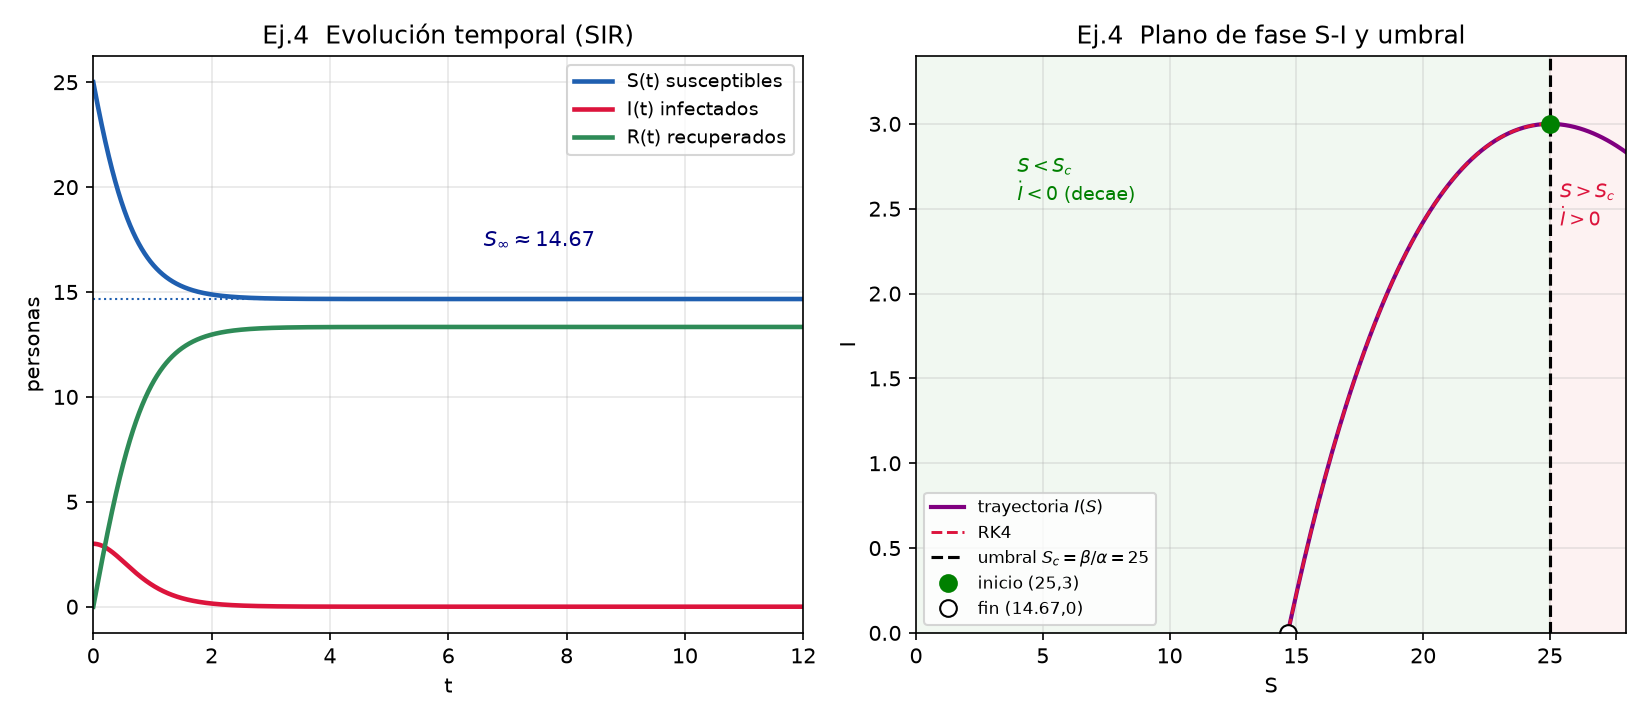
\includegraphics[width=0.99\textwidth]{ej4b_sir.png}\end{figure}

\vspace{2pt}
%==================================================================
\seccion{Resumen}

\begin{center}
\renewcommand{\arraystretch}{1.3}
\begin{tabular}{c l l}
\toprule
Ej. & Tema & Resultado clave\\
\midrule
1 & Integración numérica & Trapecio $=0.8241$; Simpson $=0.8225$ (exacto $\pi^2/12=0.8225$)\\
2 & Competencia con $\mu$ & bifurcación en $\mu=1$: $\mu<1$ gana $x$, $\mu>1$ gana $y$\\
3 & Van der Pol & origen inestable + \textbf{ciclo límite} estable único\\
4 & SIR & $S_c=\beta/\alpha=25$, $R_0=1$; $S_\infty\approx14.67$\\
\bottomrule
\end{tabular}
\end{center}

\end{document}
